\chapter{An\'alisis de resultados}

\label{Chapter4}

A lo largo del presente cap\'itulo, se analizar\'an los resultados obtenidos a partir de los experimentos planteados.
Se detallar\'an las m\'etricas obtenidas y los resultados de aplicar los modelos a los telegramas.

\section{An\'alisis de m\'etricas}

Los experimentos realizados arrojaron los resultados mostrados en el cuadro \ref{tab:metricas-experimentos}. Las
m\'etricas referidas a la capacidad de clasificaci\'on (Accuracy, $F_1$) son evaluadas sobre la partici\'on de test del
dataset de origen donde se conocen las etiquetas a ciencia cierta ($MNIST$). Por otro lado, las m\'etricas de
adaptaci\'on ($MMD$, Dist. $\mathcal{A}$) son evaluadas sobre los espacios latentes que los modelos generaron para las
particiones de test de ambos datasets. El mejor modelo es el que posea mejor capacidad de clasificaci\'on y de
adaptaci\'on.

% TODO: cambiar f1 por macro para que sea distinto a acc. que onda iou?
\begin{table}[H]
    \centering
    \begin{tabular}{cc|rrrr}
        \toprule
                                 &        & Acc.                               & $F_1$                               & $MMD$                               & Dist. $\mathcal{A}$                 \\
        AD                       & Modelo &                                    &                                     &                                     &                                     \\
        \midrule
        \multirow[c]{2}{*}{-}    & ResNet & \textbf{{\footnotesize (1)} 98.73} & \textbf{{\footnotesize (1)} 0.9873} & 0.0595                              & 1.9443                              \\
                                 & LeNet  & 98.14                              & 0.9814                              & 0.0498                              & 1.9313                              \\\hline
        \multirow[c]{2}{*}{MDD}  & ResNet & 98.58                              & 0.9858                              & 0.0569                              & 1.9031                              \\
                                 & LeNet  & {\footnotesize (3)} 98.62          & {\footnotesize (3)} 0.9862          & 0.0363                              & 1.7259                              \\\hline
        \multirow[c]{2}{*}{DANN} & ResNet & 97.52                              & 0.9752                              & 0.0153                              & 1.6383                              \\
                                 & LeNet  & 98.14                              & 0.9814                              & {\footnotesize (2)} 0.0119          & {\footnotesize (3)} 1.6231          \\\hline
        \multirow[c]{2}{*}{AFN}  & ResNet & {\footnotesize (2)} 98.68          & {\footnotesize (2)} 0.9868          & \textbf{{\footnotesize (1)} 0.0037} & \textbf{{\footnotesize (1)} 1.0047} \\
                                 & LeNet  & 98.58                              & 0.9857                              & {\footnotesize (3)} 0.0138          & {\footnotesize (2)} 1.5920          \\\hline
        \multirow[c]{2}{*}{ADDA} & ResNet & 89.18                              & 0.8918                              & 0.0225                              & 1.8691                              \\
                                 & LeNet  & 97.49                              & 0.9749                              & 0.0288                              & 1.8112                              \\
        \bottomrule
    \end{tabular}
    \caption{M\'etricas de los experimentos realizados. Entre par\'entesis se encuentra la posici\'on que ocupa dentro del top 3 de la columna.}
    \label{tab:metricas-experimentos}
\end{table}

Como era de esperarse, los modelos que fueron entrenados sin adaptaci\'on de dominio son los que mejores m\'etricas de
clasificaci\'on poseen. No obstante, sus valores de adaptaci\'on son los peores provocando que no puedan ser aplicados
en $TDS$.

El modelo que mejor combinaci\'on de clasificaci\'on y adaptaci\'on es la ResNet utilizando AFN. Cabe destacar que los
modelos LeNet entrenados con DANN y AFN obtuvieron buenas m\'etricas en general, lo que deja en evidencia que {\it no
        siempre un modelo m\'as complejo es mejor}.

Es posible aplicar los modelos sobre todos los telegramas y calcular el $IoU$ promedio por telegrama con el c\'alculo
descripto en el cap\'itulo \ref{Chapter3} y la cantidad de aciertos promedio por telegrama utilizando como etiquetas lo
transcripto en el centro de c\'omputo suponiendo que existen pocos errores en ellos.

\begin{table}[H]
    \centering
    \begin{tabular}{cc|rrr}
        \toprule
                                 &        & $IoU$ prom.     & \# aciertos prom. & \% aciertos prom. \\
        AD                       & Modelo &                 &                   &                   \\
        \midrule
        \multirow[c]{2}{*}{-}    & ResNet & 0.4494          & 4                 & 22\%              \\
                                 & LeNet  & 0.4715          & 6                 & 33\%              \\\hline
        \multirow[c]{2}{*}{MDD}  & ResNet & 0.5451          & 8                 & 44\%              \\
                                 & LeNet  & 0.5801          & 9                 & 50\%              \\\hline
        \multirow[c]{2}{*}{DANN} & ResNet & 0.6941          & 12                & 67\%              \\
                                 & LeNet  & 0.7024          & 12                & 67\%              \\\hline
        \multirow[c]{2}{*}{AFN}  & ResNet & \textbf{0.7486} & \textbf{13}       & \textbf{72\%}     \\
                                 & LeNet  & 0.6493          & 11                & 61\%              \\\hline
        \multirow[c]{2}{*}{ADDA} & ResNet & 0.6763          & 11                & 61\%              \\
                                 & LeNet  & 0.6406          & 10                & 56\%              \\
        \bottomrule
    \end{tabular}
    \caption{IoU promedio y cantidad promedio de aciertos al aplicar los modelos a cada telegrama.}
    \label{tab:iou-cant-aciertos-en-telegramas}
\end{table}

El cuadro \ref{tab:iou-cant-aciertos-en-telegramas} confirma la elecci\'on del mejor modelo realizada anteriormente.
Independientemente de qu\'e t\'ecnica de adaptaci\'on se utilice, todas presentan mejores porcentajes de aciertos
promedio que los modelos que fueron entrenados \'unicamente con $MNIST$.

\begin{figure}[H]
    \centering
    \begin{subfigure}[h]{0.43\textwidth}
        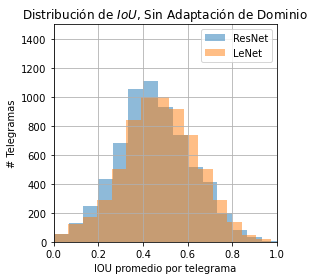
\includegraphics[height=1\textwidth]{chapter4/hist-iou-sin-da.png}
    \end{subfigure}
    \hfill
    \begin{subfigure}[h]{0.43\textwidth}
        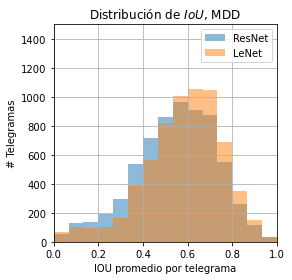
\includegraphics[height=1\textwidth]{chapter4/hist-iou-mdd.png}
    \end{subfigure}
    \hfill
    \begin{subfigure}[h]{0.43\textwidth}
        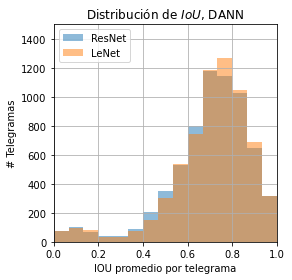
\includegraphics[height=1\textwidth]{chapter4/hist-iou-dann.png}
    \end{subfigure}
    \hfill
    \begin{subfigure}[h]{0.43\textwidth}
        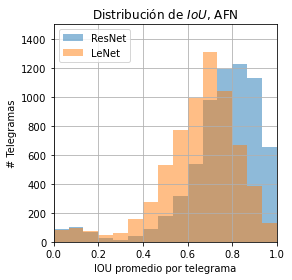
\includegraphics[height=1\textwidth]{chapter4/hist-iou-afn.png}
    \end{subfigure}
    \hfill
    \begin{subfigure}[h]{0.43\textwidth}
        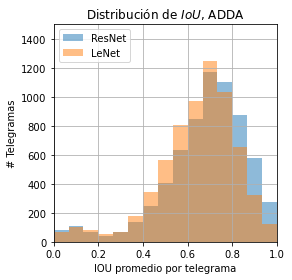
\includegraphics[height=1\textwidth]{chapter4/hist-iou-adda.png}
    \end{subfigure}

    \caption{Histogramas de la m\'etrica $IoU$ promedio por telegrama por cada par t\'ecnica AD y modelo.}
    \label{fig:histogramas-ious}
\end{figure}

Resulta interesante mencionar existen telegramas que son m\'as dif\'iciles de analizar que otros. Esto puede
evidenciarse en los histogramas de la figura \ref{fig:histogramas-ious} donde se pueden observar un conjunto de
observaciones que contienen valores entre [0, 0.2] en todos los experimentos realizados. Esto puede deberse varias
cuestiones:

\begin{itemize}
    \item Telegramas donde existen otros caracteres distintos a n\'umeros (ver ejemplo en el anexo
          \ref{anexo:telegrama-erroneo-caracteres-especiales}).
    \item Telegramas cargados de forma err\'onea (ver ejemplo en el anexo \ref{anexo:telegrama-erroneo}).
    \item Telegramas correctos pero por alguna cuesti\'on la l\'ogica de extracci\'on de d\'igitos funciona incorrectamente (ver
          ejemplo en el anexo \ref{anexo:telegrama-erroneo-caracteres-especiales}).
\end{itemize}

\section{Comparaci\'on de espacios latentes}

\lipsum[1]

\section{An\'alisis de errores}

\lipsum[1]